\chapter{Phân tích và thiết kế hệ thống}
\section{Ý tưởng đề xuất}
Các hệ thống HIDS hiện nay sử dụng cơ chế rules-based, tuy cách này
  có lợi thế về mặt thời gian, nhưng trên thực tế, các kiểu tấn công luôn thay đổi, nên
  hệ thống phát hiện được những cuộc tấn công mà chưa được biết đến là 1 điều
  cần thiết.\\\\ 
Các giải thuật gom cụm được áp dụng cho ra các kết quả khá chính xác về
  việc phân cụm sự kiện mạng, giúp cho việc đánh giá cuộc tấn công mạng có
  thể có hướng tiếp cận mới khá khả quan.\\\\ 
Từ các kết luận trên, nhóm đưa ra ý tưởng như sau: tích hợp chương trình
học máy vào trong hệ thống HIDS, để cải tiến quá trình phát hiện các hành vi
xâm nhập, từ đó nâng cao tính an toàn, tính bảo mật cho hệ thống. 
\section{Cách thiết kế hệ thống}
 \begin{figure}[h!]
	\centering 
	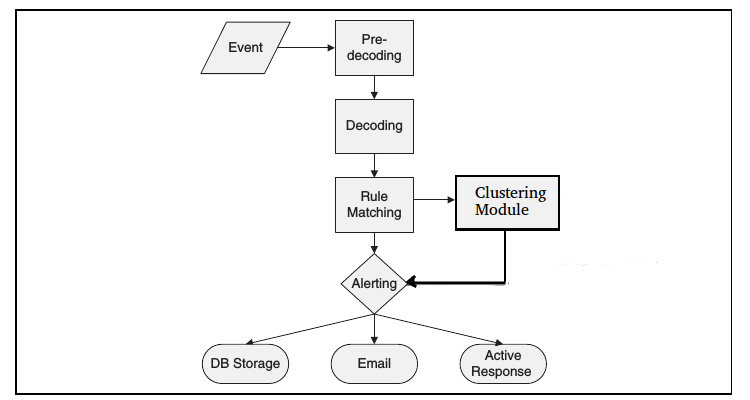
\includegraphics[width=6in,height=3in,keepaspectratio=true]{eventFlowE.png}
	\caption{Cải tiến quá trình phát hiện xâm nhập trong OSSEC}
  \end{figure}
  \subsection{Nhận sự kiện}
  Mỗi khi chương trình trong máy tính hoạt động sẽ tạo ra các log và ghi vào
  trong file log, mỗi 1 log được ghi vào đều là 1 sự kiện. Module này sẽ đảm
  nhiệm việc bắt những đoạn log này cho hệ thống, hệ thống sẽ lấy những đoạn
  log này làm input để thực hiện công việc phát hiện xâm nhập.
  \subsection{Predecode}
   Module này thực hiện nhiệm vụ rút trích các thông tin cơ bản của sự kiện. Các
   thông tin như ngày, giờ, tên chương trình của sự kiện, người dùng thực hiện
   sự kiện đều được rút trích ra, để làm thông tin kiểm tra.\\\\
   Cơ chế rút trích trong module này là sử dụng 1 chuẩn do hệ thống tự định
   nghĩa, các đoạn log của các chương trình khác nhau đều được chuẩn hóa về dạng
   chuẩn này, từ đó hệ thống sẽ rút ra những thông tin cần thiết.
  \subsection{Decode}
   Module này thực hiện nhiệm vụ rút trích các thông tin chính của sự kiện.
   Các thông tin như việc đăng nhập thành công hoặc thất bại các người dùng,
   việc nhập sai mật khẩu, việc chặn gói tin trên ACL, \ldots đều được rút trích
   trong quá trình này.\\\\
   Chúng ta có thể dễ dàng nhận thấy những thông tin trên vô cùng đa dạng. Cấu
   trúc của đoạn log hoàn toàn khác nhau, do vậy việc decode sẽ dễ ra khác nhau
   đối với từng sự kiện, dẫn đến việc mỗi 1 sự kiện đều có 1 decoder riêng.\\\\
   Việc rút trích thông tin trước hết sẽ dự vào tên chương trình mà predecoder
   đã rút trích được, sau đó sẽ tiến hành so sánh lần lượt với các decoder của
   chương trình đó để xác định decoder dùng để rút trích thông tin.\\\\
   Sau khi tiến hành quá trình rút trích, 1 dãy thông tin của
   quá trình predecode và quá trình decode được đưa vào quá trình sau để tiến hành so sánh.
  \subsection{Rule matching}
   Module này thực hiện công việc so sánh các thông tin rút trích được với những
   rule được định nghĩa sẵn trong hệ thống.\\\\
   Quá trình này trước hết sẽ dựa vào decoder được sử dụng để rút trích thông
   tin, tìm ra tất cả các rule của decoder đó. Sau đó tiến hành so sánh lần lượt
   thông tin rút trích được từ sự kiện với từng luật. Do luật trong hệ thống
   được cấu hình theo sơ đồ cây, khi trùng luật ở node cha, hệ thống vẫn tiếp
   tục so sánh với tất cả các luật ở node con. Cảnh báo được phát theo quy
   định của luật cuối cùng được so sánh trùng.\\\\
   Khi so sánh sự kiện với luật sẽ xảy ra 2 trường hợp sau: 
  \begin{enumerate}
    \item Nếu phát hiện trùng: hệ thống sẽ phát ra cảnh báo.
    \item Nếu phát hiện không trùng: dữ liệu rút trích sẽ được đưa vào
    Clustering module.
    \end{enumerate}
   \subsection{Clustering Module}
   Module này sẽ thực hiện công việc kiểm tra lần 2 cho thông tin rút trích
   được, việc kiểm tra này dựa vào học máy.\\\\
   Module sẽ nhận toàn bộ dữ liệu mà hệ thống rút trích được, dựa vào mô hình đã
   được train với tập dữ liệu tốt, gom cụm sự kiện vào 1 trong 2 cụm tấn công
   hoặc bình thường.\\\\
   Việc gom cụm này sẽ dựa vào các thuật toán gom cụm.
   \subsection{Alerting}
   Module này sẽ thực hiện nhiệm vụ phát ra cảnh báo khi phát hiện tấn công,
   được điều khiển bởi Module Rule matching và Module Clustering.
\section{Đánh giá hệ thống}
  Với mô hình trên, nhóm tạo ra hệ thống HIDS kiểu hybrid, kết hợp giữa hệ
thống Rules based và hệ thống Behavior based.\\\\ 
Các dữ liệu rút trích từ sự kiện trước hết phải thông qua
bộ so sánh rule của bản thân OSSEC, nếu sự kiện không trùng mới đi qua hệ
thống Clustering. \\\\
Như vậy, hệ thống mới vẫn giữ được tốc độ của việc phát
hiện xâm nhập trong hệ thống cũ, các dấu hiệu tấn công đã biết vẫn được sử dụng, đảm bảo
việc chính xác trong khi xét các sự kiện đã biết. Bên cạnh đó, các sự kiện không
có dấu hiệu trong rule, được kiểm tra lần 2 trong hệ thống clustering, tăng
thêm tính bảo mật.\\\\  
Ngoài ra, có thể thêm tính năng tự cập nhật rule. Một khi sự kiện được
clustering module phân vào cụm tấn công, và được người dùng xác thực về sự
tấn công đó, hệ thống có thể rút trích các thông tin của sự kiện và viết thành
rule. Sau khi được cập nhật rule, khi gặp lại sự kiện tương tự, hệ thống có thể
nhanh chóng phát hiện tấn công bằng rules.\\\\ 
Clustering module có thể thêm khả năng phân các cuộc tấn công thành nhiều cụm,
chia thành từng loại tấn công, tăng tính rõ ràng cho dữ liệu.